\documentclass[12pt,letterpaper,noanswers]{exam}
\usepackage[usenames,dvipsnames,svgnames,table]{xcolor}
\usepackage[margin=0.9in]{geometry}
\renewcommand{\familydefault}{\sfdefault}
\usepackage{multicol}
\usepackage{wrapfig}
\pagestyle{head}
\definecolor{c03}{HTML}{FFDDDD}
\header{AM 22b Class 26}{}{Apr 2: Flux, p. \thepage}
\runningheadrule
\headrule
\usepackage{graphicx} % more modern
\usepackage{amsmath} 
\usepackage{amssymb} 
\usepackage{hyperref}
\usepackage{tcolorbox}
\usepackage[utf8]{inputenc}
\usepackage{diagbox}
\usepackage{graphicx} 
\usepackage{enumitem}
\usepackage{tikz}
\tikzstyle{startstop} = [rectangle, rounded corners, minimum width=3cm, minimum height=1cm,text centered, draw=black]

\tikzstyle{process} = [rectangle, minimum width=3cm, minimum height=1cm, text centered, draw=black, fill=gray!20]
\tikzstyle{decision} = [ellipse, minimum width=3cm, minimum height=0.5cm, text centered, draw=black, fill=white!30]
\tikzstyle{arrow} = [thick,->,>=stealth]
\usetikzlibrary{shapes.geometric, arrows}
\pagenumbering{arabic}

\usepackage[numbered,autolinebreaks,useliterate]{mcode}

\newcommand{\mb}[1]{\underline{#1}}

\begin{document}
 \pdfpageheight 11in 
  \pdfpagewidth 8.5in




% I need to review the torus trajectories...

\begin{itemize}
% \item There is a pre-class assignment (20 minutes of videos + a few WeBWorK exercises) due at 10am this Monday.  It is available on Canvas.
\itemsep0em
\item Quiz 04 will be available on Gradescope from $\sim$3pm today until Sunday at 6pm ET.
\item There will be a skill check on Monday (Skills C25 and C26).
\item Problem Set 08 is posted (due Thursday April 8th at 6pm ET).
\item For your quizzes, a few students have asked whether there is a way to make up for a satisfactory quiz with a lower score.  To address this, I will count your lowest quiz score as worth only half of the rest of the quizzes (the weighting on all quizzes will change).
\end{itemize}

\hrule
\vspace{0.2cm}

% partial derivatives, gradient
% local linearity, differential, directional deriv
% 2nd order partials + equations with partials

\noindent\textbf{Big picture}

Today (and part of next week) we will compute flux integrals, where we calculate how much the vector field pushes through a curve or surface.  This requires learning how to compute surface integrals (integrals over an arbitrary surface in $3$-space).  For the flux out of a closed surface (or curve) we will have a theorem similar to Green's theorem, where we will integrate the flux density over a region to find the flux out the boundary of the region.

\vspace{0.2cm}
\hrule
\vspace{0.2cm}

\noindent\textbf{Skill Check C26 Practice}
Identify the sign of the flux of $\mb F = x\mb j$ through the surface $S$, where $S$ is the piece of the plane $y = 2$ with $-3\leq x \leq 0, 0\leq z\leq 2$ and $S$ is oriented with its normal vector pointing towards the $xz$-plane.  Provide brief justification.
\vspace{0.2cm}
\hrule
\vspace{0.2cm}

\noindent\textbf{Skill Check C26 Practice Solution}

On the region $S$, $x\mb j$ points in the negative $\mb j$ direction because $x \leq 0$.

$S$ is a piece of the plane $y = 2$ so its normal vector is $\mb j$ or $-\mb j$.

We've been told to orient $S$ so that the normal vector points towards the $y = 0$ plane, so $-\mb j$.

The vector field and the normal vector are pointing in the same direction.  The flux will be positive.

\vspace{0.2cm}
\hrule
\vspace{0.2cm}

\noindent\textbf{Teams}
\begin{multicols}{2}

1.  student names
\end{multicols}
\vspace{0.2cm}
\hrule
\vspace{0.2cm}
\noindent\textbf{Example: sign of flux}

For each of the closed curves below, identify the sign of the flux, $\oint_C \mb F\cdot \mb n\ ds$.  \emph{By convention, $\mb n$ is a unit vector pointing outward outward when the curve is a closed curve}.

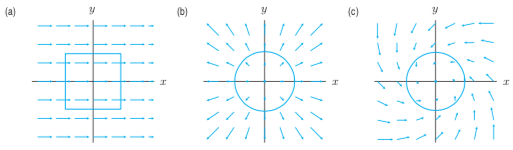
\includegraphics[scale=0.8]{img/C24p1.png}

\vspace{0.5in}


\begin{tcolorbox}
\begin{itemize}
\itemsep0em
    \item $\displaystyle\int_C \mb F\cdot \mb T ds$ has a function of integration $\mb F \cdot \mb T$, the projection of the vector field onto the curve $C$.  This type of line integral can be used to compute the work done by a force or the circulation of a vector field.
    \item $\mb T$ is a unit tangent vector to $C$, with $\mb T ds = d\mb r = dx\mb i + dy\mb j$.  In $2$-space, let $\mb n$ be a unit normal vector to $C$, so $\mb n ds = dy\mb i - dx\mb j$ or $\mb n ds = -dy\mb i + dx\mb j$.  When $C$ is a closed curve, choose $\mb n$ to point outward.  Otherwise, you'll be told in the problem which normal vector to choose (there is not a convention).
    \item Consider $\displaystyle \int_C \mb F\cdot \mb n ds$.  The function of integration is the component of the vector field perpendicular to $C$, so this is measuring the push of the vector field across the curve.  For $\mb F$ a velocity vector field, this integral yields a \textbf{flux}.
    \item A \textbf{flux} is an amount transported across a curve or surface per unit time.
\end{itemize}
\end{tcolorbox}

\vspace{0.2cm}
\hrule
\vspace{0.2cm}

\noindent\textbf{Flux across a surface} \S 19.1



\begin{tcolorbox}
\begin{itemize}
\itemsep0em
    \item A \textbf{flux} is an amount transported through a region per unit time.  The amount could be a volume or mass per unit time crossing a plane or surface, a flux of particles, or even a flux of heat.
    %\item A \textbf{flux density} is an amount transported per unit time per unit area.  The integral of a flux density over a surface yields the flux through that surface.
\end{itemize}


% For example, think of a stretch of highway (moving one way) with no entrance or exit ramps.  Cars enter at one end of the highway and leave at the other.  The rate of cars entering the stretch of road is a flux of cars per unit time, and the rate of cars leaving is a flux of cars per unit time.  Since cars have only one way to appear on the road (they come in on the left) and one way to leave (they drive off on the right), the time evolution of the number of cars on the stretch of highway is related to the flux of cars entering and leaving.
\end{tcolorbox}



% \noindent\textbf{Estimating how much is crossing a surface.}  In the image below, a little boat (an `acoustic Doppler current profiler') is using radar to measure velocity vectors for flowing water.  Those velocity measurements are used to estimate how many cubic feet per second of water are flowing downstream.

% \begin{itemize}
%     \item To estimate how many cubic feet per second are flowing downstream, we could think of this via a sum.  It would be the sum of the flux through each grid box shown below.
%     \item We would then need a method for estimating the flux through a small box from the velocity vectors.
%     \item In place of a sum, we will integrate the flux per unit area (the flux density) over a surface.
% \end{itemize}
% \vspace{0.3cm}

% \includegraphics[width=4in]{img/C29p1-18.png}

% \url{https://water.usgs.gov/edu/streamflow2.html}(Accessed Nov 11, 2018)

\noindent\textbf{Reasoning about processes within a region}.  Consider the net flux of oxygen into your brain, through your neck.  Do you expect more oxygen to pass upward to your head than passes back downward towards your body?
\vspace{0.8in}

Note: If you have a process where more of something is entering a region per unit time than leaves the region, the substance could be accumulating in the region or might be used within the region.

\vspace{1cm}




%\noindent\textbf{Flux through a flat surface}.
% \begin{itemize}
%     \item To reason about flux, think of the vector field, $\mb v$, as a velocity vector field.
%     \item At the surface, if a unit normal vector to the surface is $\hat n$, each velocity vector can be written as a sum of a component pushing through the surface ($(\mb v\cdot \hat n) \hat n$) and a component pushing along (tangent to) the surface ($\mb v-(\mb v\cdot \hat n) \hat n$).
%     \item For a flat surface with area vector $\mb A$ and a constant vector field, $\mb v$, $\mb A = \Vert \mb A\Vert\hat n$ and the flux of the vector field through the surface is $(\mb v\cdot \hat n)\Vert \mb A\Vert = \mb v\cdot \mb A$
%     \item For a curved surface or for a vector field changing in space, think of the flux as $\sum \mb v\cdot \Delta \mb A$ where $\Delta \mb A$ is the area vector for a small piece of the surface (small enough that it makes sense to approximate $\mb v$ as constant and the piece as flat). 
%     \item The orientation of $\mb A$ relative to the velocity of the fluid determines the sign of the flux.
% \end{itemize}

\noindent\textbf{Example (sign of the flux through a flat surface)}

In the image below, the orange vector is the area vector for the surface, where an \textbf{area vector}, $\mb A$, is a vector that points normal to a flat surface, $S$, with $\Vert \mb A \Vert = \text{Area}(S)$.


What is the sign of the flux through this surface?  Use the orientation of the area vector to denote positive flux.


%\includegraphics[width=2.5in]{img/C29p2-18.png}\hfill
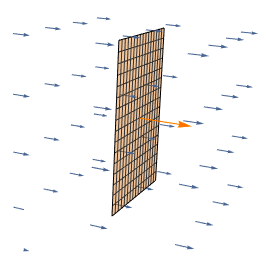
\includegraphics[width=2.5in]{img/C29p3-18.png}


\noindent\textbf{Example (sign of flux)}.  Five oriented surfaces are shown below.  For each oriented surface, identify the vector fields that give a positive flux:
\[\mb F_1 = x\mb j\quad \mb F_2 = x\mb k\quad \mb F_3 = -y\mb k\quad \mb F_4 = y\mb j\quad \mb F_5 = -z\mb i\quad \mb F_6 = (z+x)\mb i.\]

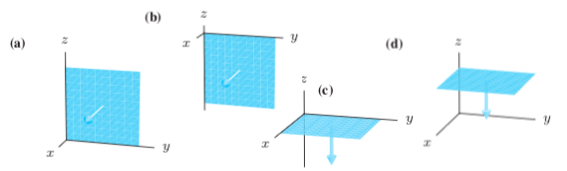
\includegraphics[width=\linewidth]{img/C29p4-18.png}

\emph{pollQ}

\vspace{0.2cm}
\hrule
\vspace{0.2cm}

\noindent\textbf{Using an integral to compute flux} \S 19.1
\begin{tcolorbox}
\begin{itemize}
\itemsep0em
    \item The \textbf{flux integral} of the vector field $\mb F$ through the surface $S$ is $\displaystyle \int_S \mb F\cdot d\mb A = \int_S \mb F \cdot \mb n dS$ where $\mb n$ is a unit vector normal to the surface and $dS$ is a piece of the surface.
    \item If $S$ is a closed surface oriented outward, then we say the flux through $S$ is the \textbf{flux out of $S$}.
%    \item Let $\Delta S$ be a small patch of the surface $S$.  If it has unit normal vector $\mb n$ and area $\Delta A$ then it will have area vector $\Delta \mb A = \mb{ n}\Delta A$.  We say that $\mb F\cdot \mb{n}$ is the \textbf{flux density}, and can write the flux integral as $\displaystyle \int_S \mb F\cdot d\mb A = \int_S \mb F\cdot \mb n\ dA$
\end{itemize}
\end{tcolorbox}

\noindent\textbf{Worked example (spherical symmetry).}  

Calculate the flux integral $\displaystyle \int_S \mb r\cdot d\mb A$ where $S$ is the sphere of radius $3$ centered at the origin.
\begin{itemize}
    \item By convention, a closed surface is oriented outward.
    \item This sphere is $x^2+y^2+z^2 = 3$.  The vector $\underline n = \langle 2x,2y,2z\rangle$ is an outward normal to the sphere at the point $(x,y,z)$.
    \item $d \mb S = \hat{\underline n} dS$ where $\hat{\underline n}$ is an outward unit normal vector ($\hat{\underline n} = \langle x/3,y/3,z/3\rangle$) on the patch $d \mb S$ and $d S$ is the area of the patch.  \emph{$d\underline S$ encodes the orientation of the patch and its area.}
    \item $\mb r$ and $\hat{\underline n}$ point in the same direction
    \item $\mb r\cdot d\mb S = \Vert \mb r\Vert d S$.  On the sphere, $\Vert \mb r\Vert = 3$.
    \item $\displaystyle \int_S \mb r\cdot d\mb S =\int_S 3 dS =  3\cdot(\text{Surface area of sphere})$
\end{itemize}
\vspace{2.5in}

\noindent\textbf{Problem}.  Let $S$ be part of a cylinder centered on the $y$-axis.  Explain why the vector fields $\mb F$ and $\mb G$ have the same flux through $S$ where $\displaystyle \mb F = x\mb i + 2yz\mb k$, $\displaystyle \mb G = x\mb i + y\sin x\mb j + 2yz\mb k$.


\vspace{1.5in}

\noindent\textbf{Worked example (flux integral)}.  Set up an integral to find the flux of $\mb F = -z\mb i$ through the surface $S$ shown in (a) above.  $S$ is oriented in the $\mb i$ direction with $x = 0, 0\leq y\leq L, 0\leq z\leq L$.

\begin{enumerate}
\itemsep0em
    \item $d\mb A$ for the surface is $\mb i dydz$.
    \item $\mb F\cdot d\mb A$ on the surface is $-zdydz$.
    \item Setting up an integral over the region in $xz$-space corresponding to the surface, $\int_S \mb F\cdot d\mb A = \int_0^L\int_0^L -z dy dz$
\end{enumerate}


\vfill

\eject
\vspace{0.2cm}
\hrule
\vspace{0.2cm}

\noindent\textbf{Computing a surface integral: surface area} \S 19.2
\begin{tcolorbox}
\begin{itemize}
\itemsep0em
    \item To find the \textbf{surface area} of a surface $S$, compute the integral $\int_S dS = \int_S \Vert d\mb A\Vert$, where $dS$ are small pieces of the surface $S$.  Our course text uses $dA$ rather than $dS$ so would denote this integral $\int_S dA$.
    \item Let $S$ be a piece of the graph $z = f(x,y)$ with projection $R$ in the $xy$-plane.  It is convenient to set up an integral over $R$ (the projection), but we have to account for the difference in size between pieces of $R$ and pieces of $S$.  The size of a piece of the surface and the size of its shadow in the $xy$-plane is not the same.
    \item Let $\Delta \mb A$ be the area vector of a small piece of $S$.  $\displaystyle \Delta \mb A \approx (-f_x\mb i - f_y\mb j + \mb k)\Delta x\Delta y$, where $\Delta x\Delta y$ is the shadow of $\Delta \mb A$ in the $xy$-plane.  $dS = \Vert d\mb A\Vert$, so we have $\displaystyle\int_S dS = \int_R \Vert \langle -f_x, -f_y, 1\rangle \Vert dA$ where $dS$ is a piece of $S$ and $dA$ is a piece of $A$.
    \item \textbf{Notation challenge}.  In the expression $\int_R dA$ with region of integration $R$ (a piece of the $xy$-plane), $\Delta A = \Delta x\Delta y$.  In the expression $\int_S dA$ with region of integration $S$ (a surface embedded in $3$-space) $\displaystyle \Delta A = \Vert \Delta \mb A\Vert = \left(\sqrt{f_x^2+f_y^2+1}\right)\Delta x\Delta y$.   
\end{itemize}


\end{tcolorbox}

\noindent\textbf{Illustration: area of surface}.  Think of the surface below as being made up of parallelograms (diagram on left), where one side corresponds to $\Delta x$ and the other side to $\Delta y$.  $\mb v_1 \approx \langle \Delta x, 0, f_x \Delta x \rangle$ and $\mb v_2 \approx \langle  0,\Delta y, f_y\Delta y\rangle$.

In the middle image, each parallelogram is drawn just above its corresponding box in the $xy$-plane.  For the surface area, we'll sum over the boxes in the $xy$-plane, and for each of those boxes, we'll sum the area of the parallelogram above the box.  

In the image on the right, the area vectors are shown (scaled down, so the length isn't quite right), for a few of the parallelograms.  $\Delta \mb A \approx \mb v_1\times \mb v_2 = (-f_x\mb i - f_y\mb j + \mb k)\Delta x\Delta y$.  $\Delta S \approx \Vert \mb v_1 \times \mb v_2\Vert = \left(\sqrt{f_x^2+f_y^2+1}\right)\Delta x\Delta y$.

% \includegraphics[width=0.7\linewidth]{img/C30p1-18.png}
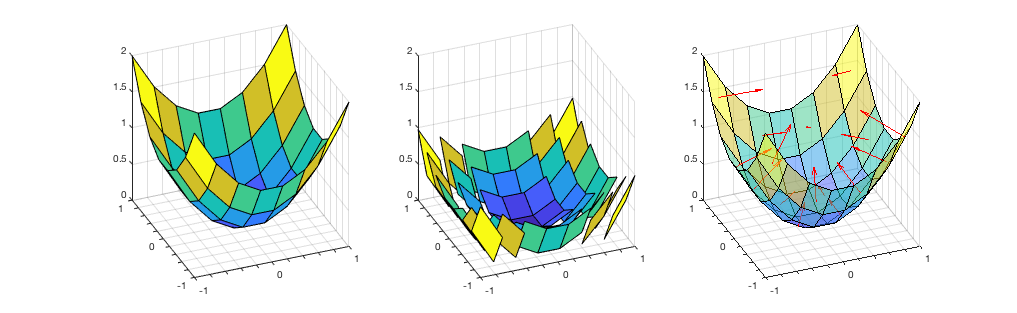
\includegraphics[width=1\linewidth]{img/C30p4-18.png}

\noindent\textbf{Example (surface area)}.  Let $S$ be the part of the surface $z = x^2+y^2$ above the disk, $R$, of radius $2$ centered at the origin in the $xy$-plane.  Find the surface area of $S$.

\begin{enumerate}
\itemsep3em
    \item Find $f(x,y)$ so that $z = f(x,y)$ (making $S$ a piece of the graph $z = f(x,y)$). %Let $f(x,y) = x^2+y^2$, so $S$ is a piece of the graph $z = f(x,y)$.
    \item Find $f_x, f_y$.  %$f_x = 2x$, $f_y = 2y$, $\left\Vert -f_x\mb i -f_y\mb j + \mb k\right\Vert$ $= \sqrt{4x^2+4y^2+1} = \sqrt{4r^2+1}$.
    \item Find $dS$ in terms of $dA$ (where $dA$ is a piece of the $xy$-plane and $dS$ is a piece of the surface).  %$dS = \Vert d \mb A \Vert = \sqrt{4r^2+1} dA$ where $dS$ is a piece of the surface $S$ and $dA$ is a piece of its shadow in the $xy$-plane, $R$.
    \item Rewrite $\int_S dS$ as an integral over the region $R$ in the $xy$-plane. %$\displaystyle \int_S dA = \int_R \left(\sqrt{4r^2+1}\right)dA$.  Note that in this equation $dA$ is indicating a piece of the paraboloid on the left hand side and is indicating a piece of the disk on the right hand side.
    \item Compute that integral to find the surface area.  %Set up an iterated integral for $\int_R \left(\sqrt{4r^2+1}\right)dA$.  
    \vspace{1in}
    
    
\end{enumerate}
\begin{verbatim}
    int(int(sqrt(4*r^2+1)*r,r,0,1),theta,0,2*pi)
    % answer is (pi*(5*5^(1/2) - 1))/6
    \end{verbatim}

\noindent\textbf{Example (surface area)}.  Set up an iterated integral to find the area of $S$ where $S$ is the piece of the surface $z = xy$ whose projection onto the $xy$-plane is the disk $x^2+y^2\leq 1$.

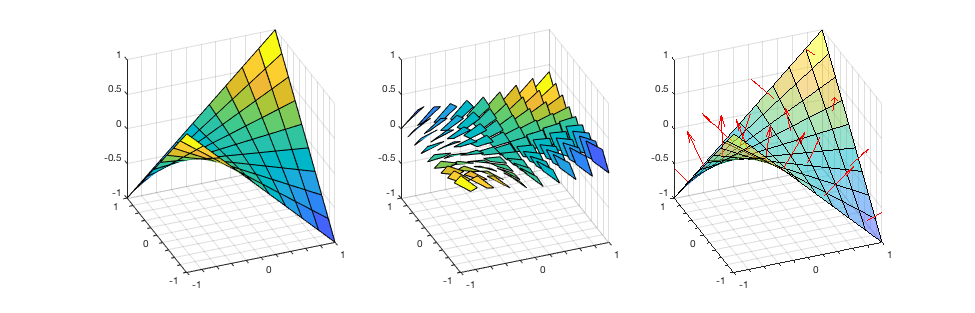
\includegraphics[width=1\linewidth]{img/C30p5-18.png}

% \includegraphics[width=0.7\linewidth]{img/C30p2-18.png}



\vspace{1.5in}
\eject

\vspace{0.2cm}
\hrule
\vspace{0.2cm}

\noindent\textbf{Integrating a function on a surface: finding a flux} \S 19.2
\begin{tcolorbox}
\begin{itemize}
\itemsep0em
    \item To set up a flux integral, use $\displaystyle \int_S \mb F\cdot d\mb A = \int_S \mb F \cdot \mb n\ dS$ where $\mb n$ is a unit vector normal to the surface and $dS$ is a piece of the surface:
    \item When $S$ is a part of the graph $z = f(x,y)$ oriented upward, $\displaystyle d\mb A = \mb n dS = \frac{\langle -f_x, -f_y,1\rangle}{\sqrt{f_x^2+f_y^2+1}} dS = \frac{\langle -f_x, -f_y,1\rangle}{\sqrt{f_x^2+f_y^2+1}}\sqrt{f_x^2+f_y^2+1} dA = \langle -f_x, -f_y,1\rangle dA$, where $dA$ is a piece of $R$, and $R$ is the projection of the surface $S$ onto the $xy$-plane (it's "shadow").  \item When $S$ is a part of the graph $z = f(x,y)$ oriented upward, $\displaystyle \int_S \mb F\cdot d\mb A = \int_R \mb F(x,y,f(x,y))\cdot \langle -f_x, -f_y, 1\rangle dA$.  \emph{Notice that the first integral is over the original surface $S$ and the second is over the $xy$-plane projection, $R$.}
 %   \item We will look at other cases (where $S$ cannot be written as a part of a graph) on a different day.
\end{itemize}


\end{tcolorbox}


\vspace{0.2cm}
\hrule
\vspace{0.2cm}
\noindent\textbf{Example (setting up a flux integral through a graph)}.

Compute the flux of $\mb F = z\mb k$ through $S$ where $S$ is the portion of the plane $x+y+z=1$ in the first octant, oriented upward.

\begin{enumerate}
\itemsep3em
    \item Find $f(x,y)$ so that $z = f(x,y)$ (making $S$ a piece of the graph $z = f(x,y)$).  %Rewrite $x+y+z = 1$ as $z = 1-x-y$, so $z=f(x,y)$ with $f(x,y) = 1-x-y$.
    \item Find $d\mb A = \langle -f_x, -f_y, 1\rangle dA$ for this surface. %Find $\mb n = \langle -f_x,-f_y,1\rangle$.  $\mb n = \langle 1, 1, 1\rangle$ for this surface.
    \item Compute $\mb F(x,y,z)\cdot \langle -f_x, -f_y, 1\rangle$ (this is sometimes $0$ or constant so is worth doing first).  %We have $\mb F\cdot \mb n = z.$
    \item Find $\mb F(x,y,f(x,y))\cdot \langle -f_x, -f_y, 1\rangle$, so that $\mb F$ is being computed on the surface $S$. %, so sub $f(x,y)$ in place of $z$.  We find $\mb F(x,y,f(x,y))\cdot \mb n = 1-x-y$.
    \item Identify the region $R$ in the $xy$-plane corresponding to $S$.  %Here, $x,y,z\geq 0$.  When $z = 0$, $x+y = 1$ so in the first octant the plane is above a triangle bounded by $x =0, y=0, x+y=1$.
    \item Set up the integral $\displaystyle \int_R \mb F\cdot \mb n dA$.  %In this case we have $\displaystyle\int_0^1\int_0^{1-x}(1-x-y)dydx.$
    \vspace{1in}
\end{enumerate}

\noindent\textbf{Example (setting up a flux integral through a graph)}.

Set up an integral to compute the flux of $\mb F$ through $S$ where $\mb F = \ln(x^2)\mb i + e^x\mb j + \cos(1-z)\mb k$ and $S$ is the part of the surface $z = -y+1$ above the square $0\leq x\leq 1$, $0\leq y\leq 1$, oriented downward.

\vspace{2in}





\end{document}